\documentclass[../../dissertation.tex]{subfiles}
\begin{document}

\subsection{Grover}
Like it was seen in section \ref{sec:chapGrover}, Grover's algorithm is a quantum alternative to unstructured search problems. Consider the case of finding element $x_0$ out of an unordered list of size $N$. Worst case scenario, a classical algorithm would need to check every element of the list, requiring $N$ steps.\par
The first stage of Grover's algorithm is to create an uniform superposition of all states in the system
\begin{equation}
	\ket{\Psi_0}  = \frac{1}{\sqrt{N}}\sum_{x=0}^{N-1} \ket{x}.
\end{equation}
Next is the application of the Grover iteration process, which starts with an oracle that adds a negative phase to the solution states
\begin{equation}
        \mathcal{O}\ket{x} = (-1)^{f(x)}\ket{x}.
\end{equation}
This operator can be seen as an identity matrix with negative entries corresponding to the solution states, and the operator can be rewritten as 
%TODO: Reescrever com o somatorio dos estados marcados?
\begin{equation}
	\mathcal{O} = I - 2\sum_{m\in M} \ket{m}\bra{m}.
	\label{eq:groverQiskitOracle}
\end{equation}
where $I$ is the identity matrix and $M$ is a set of solutions where $f(m) = -1$. The matrix associated with this operator will be
\begin{equation}
	\mathcal{O} = 
	\begin{pmatrix}
		(-1)^{f(0)} & 0 & \cdots & 0\\
	        0 & (-1)^{f(1)} & \cdots & 0\\ 
	        \vdots & 0 &  \ddots & \vdots\\ 
		0 & 0 & \cdots &  (-1)^{f(N-1)}
	\end{pmatrix}.
	\label{eq:oracleMatrixQiskit}
\end{equation}
%TODO: Mencionar que o grover se extende a toda a categoria de problemas que envolvam aquela matriz.
The second part of the iteration is an amplitude amplification process by means of the diffusion operator 
\begin{equation}
        %TODO: Decidir se mantenho os H's.
        \mathcal{D} = (2\ket{\Psi_0}\bra{\Psi_0} - I) = H^{\otimes n}(2\ket{0}\bra{0} - I)H^{\otimes n}.
	\label{eq:groverQiskitDiffusion}
\end{equation}
The unitary operator that describes the Grover iteration process will then be
\begin{equation}
        \mathcal{U} = \mathcal{D}\mathcal{O}.
\end{equation}\par
%TODO: Se calhar desenhar o circuito sem ser no qiskit onde e obvio que se aplicam as cenas varias vezes?
As was shown in section \ref{sec:chapGrover} this iteration process will be done several times, depending on the number of elements. Optimal probability of success finding a single solution will be reached after $\floor{\frac{\pi}{4}\sqrt{N}}$ steps, and $\floor{\frac{\pi}{4}\sqrt{\frac{N}{K}}}$ for $K$ solutions, which is a quadratic gain when compared to the classical case.\par

\begin{figure}[!h]
	\centering
	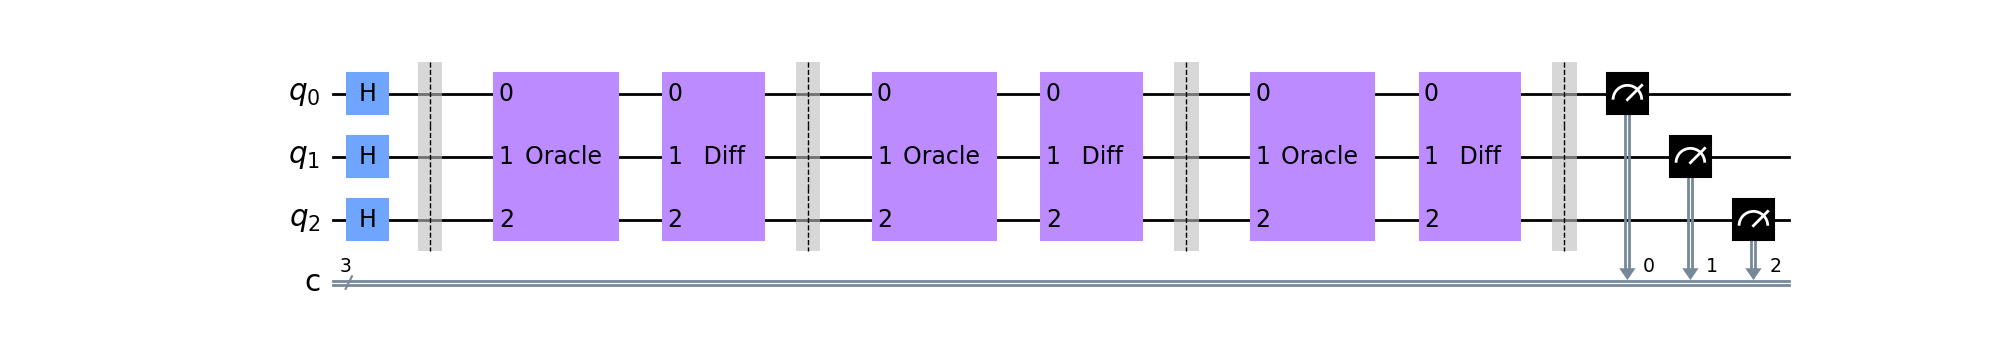
\includegraphics[scale=0.30]{img/Qiskit/GroverQiskit/Circuits/GroverQiskitCirc_N3_M4_S3.png}
	\caption{Temp}
	\label{fig:groverCircuitQistkit}
\end{figure}\par

Consider the $3$ qubit case, where $N=8$ and solution state $\ket{4}$. The optimal number of iterations is approximately $2$, and figure \ref{fig:groverCircuitQistkit} is the circuit for $3$ iterations.
%TODO:Melhorar 
The system starts with the creation of an uniform superposition state, which means applying Hadamard gates to each qubit. 
\begin{figure}[!h]
	\centering
	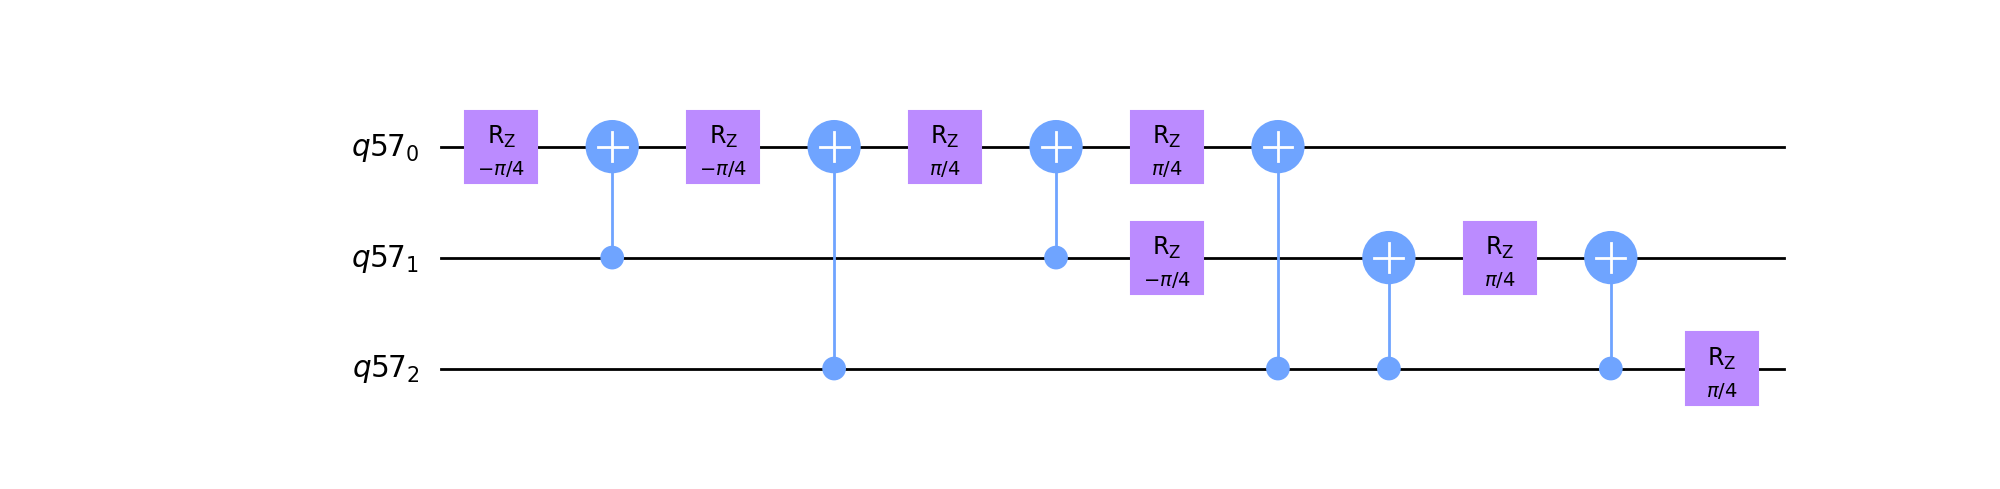
\includegraphics[scale=0.30]{img/Qiskit/GroverQiskit/Circuits/GroverQiskitCircOracle_N3_M4_S3.png}
	\caption{Temp}
	\label{fig:groverOracleCircuitQistkit}
\end{figure}
Immediately following the barrier, the first operator of the iteration process is the oracle, which is shown in figure \ref{fig:groverOracleCircuitQistkit}. 
Because the oracle operator is simply the identity matrix with negative entries corresponding to the solution states, it can be simply translated into a circuit by means of the diagonal function in Qiskit. The last part of the iteration is the diffusion operator, whose circuit is shown in figure \ref{fig:groverDiffCircuitQistkit}.

\begin{figure}[!h]
	\centering
	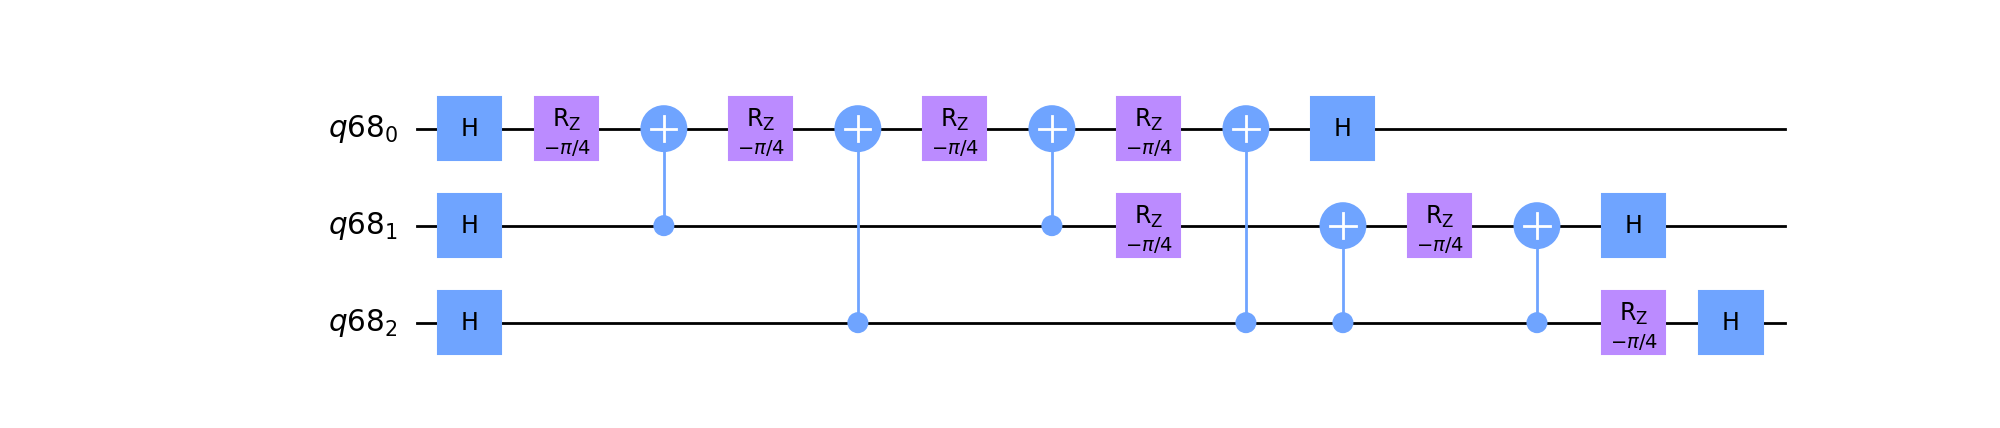
\includegraphics[scale=0.30]{img/Qiskit/GroverQiskit/Circuits/GroverQiskitCircDiff_N3_M4_S3.png}
	\caption{Temp}
	\label{fig:groverDiffCircuitQistkit}
\end{figure}\par
%TODO Isto esta muito fraco. 
Comparing equations \ref{eq:groverQiskitOracle} and \ref{eq:groverQiskitDiffusion}, it is easy to see why figures \ref{fig:groverOracleCircuitQistkit} and \ref{fig:groverDiffCircuitQistkit} are very similar. The diffusion circuit will simply be the oracle circuit for state $\ket{0}$ in between Hadamard operations.

%TODO: Escrever mais
The results of measurement are shown in figure \ref{fig:groverQiskitDist}. As was expected, maximum probability for the marked element was reached after $2$ iterations and it decreases in subsequent steps.
\begin{figure}[!h]
	\centering
	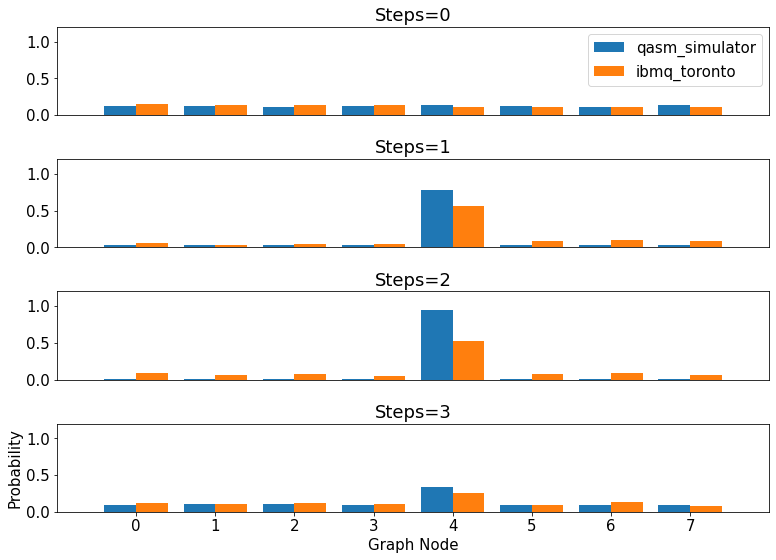
\includegraphics[scale=0.40]{img/Qiskit/GroverQiskit/GroverQiskitSearch_N3_M4_S0123}
	\caption{Temp}
	\label{fig:groverQiskitDist}
\end{figure}
%
\subsection{Coined}
As previously done in section \ref{sec:chap3CoinedSearch}, this chapter aims to expand the coined quantum walk model incorporating concepts like the oracle and diffusion operator of the Grover algorithm. In fact, for the complete graph case, the coined qua::ntum walk and Grover's algorithm are equivalent.\par
The unitary evolution operator is
\begin{equation}
        U' = S (\mmathcal{O} \otimes G),\label{eq:modifiedEvoCoinedQiskit}
\end{equation}
%TODO: Relembrar equacoes para cada um dos operadores? Parece me desnecessario.
as was defined in equation \ref{eq:modifiedEvoCoined}, where $S$ is the flip-flop shift operator, $\mathcal{O}$ is the oracle operator and $G$ is the Grover diffusion as a coin operator.\par
Considering the case of a complete graph with size $N=2^3=8$, the circuit will be as in figure

the shift operator will no longer be described by a succession of increment and decrement gates. 
%
%\begin{figure}[!h]
%	\centering
%	\includegraphics[scale=0.40]{img/Qiskit/CoinedQuantumWalk/Search/CoinedQiskitSearch_N4_M1_S01234}
%	\caption{Probability distribution for the staggered quantum walk on a line after 50 steps, with initial condition $\ket{\Psi(0)}=\frac{\ket{0}+\ket{1}}{\sqrt{2}}$, for multiple angles.} 
%	\label{fig:fig5}
%\end{figure}

%TODO: Fazer com outra moeda usando u3 com valores intermedios entre pi/2 ou pi/4
\subsection{Continuous}
\subsection{Staggered}

\end{document}
